\question[4]
a. Zeichne den Baum. \\
b. Traversiere den Baum in inorder, preorder und postorder
\begin{lstlisting}
...g
..d
.c
..b
a
...k
..i
...j
.e
..f
\end{lstlisting}

\begin{solutionbox}{6cm}
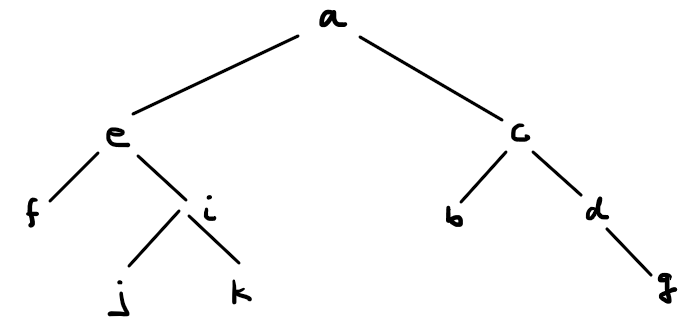
\includegraphics[height=3cm]{\pfad/Baum/Aufgaben/traverse_02/traverse_02.png}
\begin{lstlisting}
a. inorder: f e j i k a b c d g
b. preorder: a e f i j k c b d g
c. postorder: f j k i e b g d c a
\end{lstlisting}
\end{solutionbox}
